\section{Połączenie systemów}
\begin{figure}[H]
	\centering
	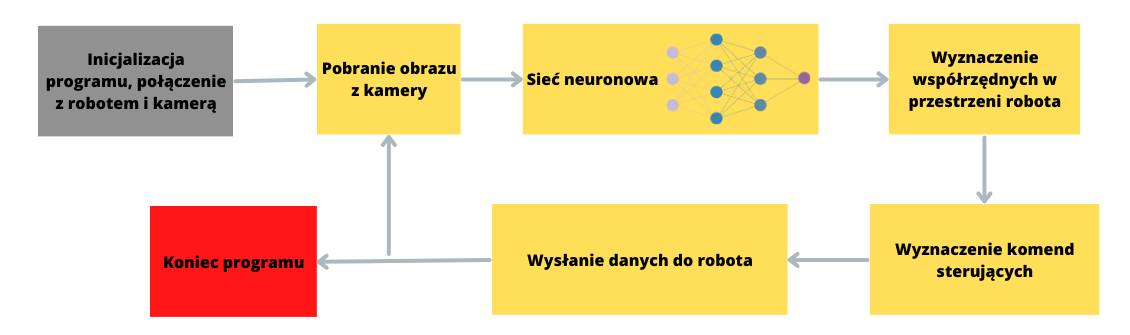
\includegraphics[width=16cm]{pages/siecIRobot/zdjecia/schematAlgorytmu.png}
	\caption{Ogólny schemat działania algorytmu}
	\label{rys:algorytmSterowania}
\end{figure}
Jak widać na algorytmie sterowania z rysunku \ref{rys:algorytmSterowania}, program w pierwszej kolejności inicjalizuje potrzebne komponenty
takie jak: kamera, połączenie z robotem oraz wczytanie wybranego modelu sieci neuronowej.
Po uruchomieniu głównej pętli algorytmu, pobierany jest obraz z kamery, który przekazywany jest do sieci neuronowej realizującej 
detekcję obiektów. Po wykryciu obiektów, wybierany jest docelowy, a następnie na podstawie jego pozycji wyznaczana jest komenda odpowiadająca 
za przesunięcie karetki robota. Cały proces jest zapętlony aż do momentu zatrzymania przez użytkownika. 
\subsection{Wykonana aplikacja kliencka}
Program obsługujący komunikacje z robotem i kamerą oraz uruchomienie sieci neuronowej wykonano w Matlab'ie i dodatku AppDesigner, 
który pozwala na zbudowanie graficznego interfejsu użytkownika i uruchamianie wytrenowanych modułów z siecią neuronową. 
\begin{figure}[H]
	\centering
	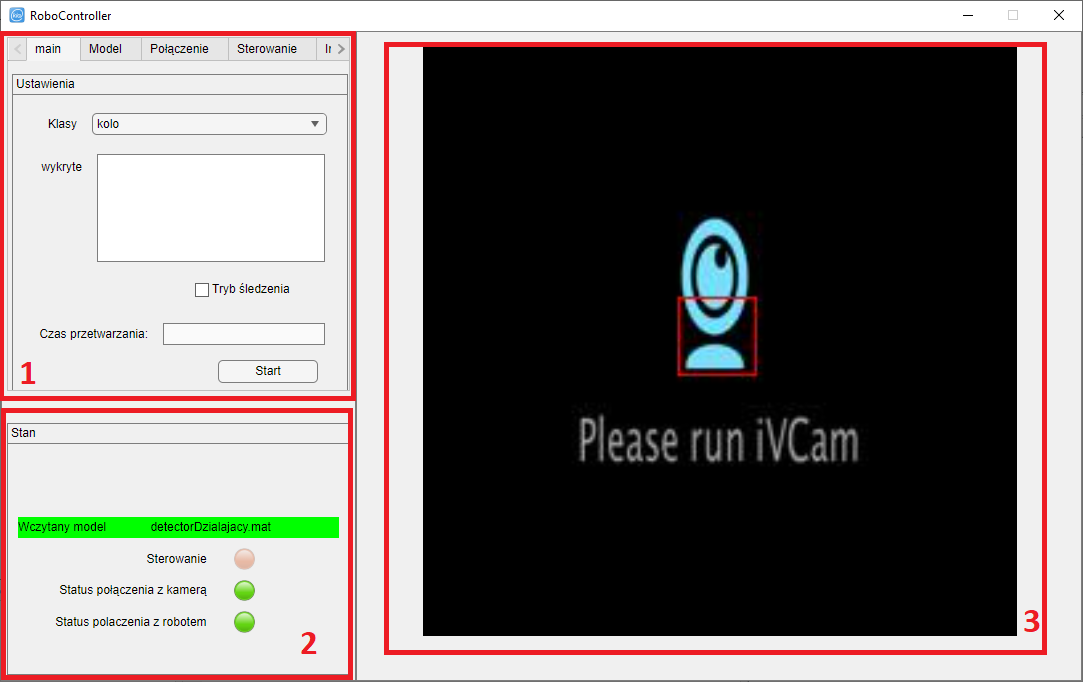
\includegraphics[width=12cm]{pages/siecIRobot/zdjecia/program/programCaly.png}
	\caption{Widok wykonanego programu}
	\label{fig:schematSterujacy}
\end{figure}
Na rys. \ref{fig:schematSterujacy} widoczne jest główne okno aplikacji. Możemy wyróżnić trzy odrębne sekcje,
odpowiadające kolejno za ustawienia sterowania, podgląd stanu poszczególnych modułów oraz podgląd obrazu i nałożonych na niego wyników sieci.
\begin{figure}[H]
	\centering
	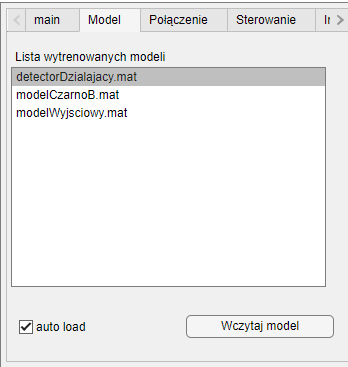
\includegraphics[height=4.5cm]{pages/siecIRobot/zdjecia/program/programUstModel.png}
	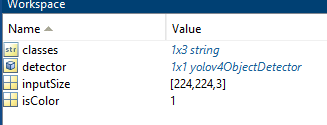
\includegraphics[height=4cm]{pages/siecIRobot/zdjecia/program/daneModeluSieci.png}
	\caption{Wczytanie danych modelu i jego struktura}
\end{figure}
Program pozwala na wczytanie wybranego pliku z modelem i jego ustawieniami. Opcja 'auto load' oznacza,
że model zostanie wczytany automatycznie zaraz po uruchomieniu aplikacji co przyśpieszyło proces testowania programu. 
Plik przechowuje wytrenowaną sieć neuronową i waży około 233Mb co oznacza, że ładowanie powoduje znaczne spowolnienie programu przy starcie.
\begin{figure}[H]
	\centering
	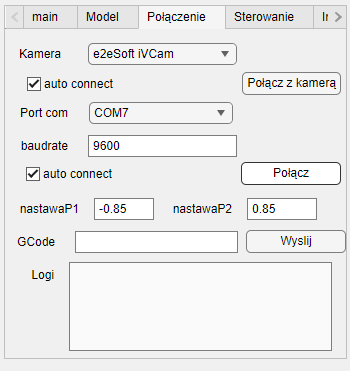
\includegraphics[height=6.5cm]{pages/siecIRobot/zdjecia/program/programUstPolaczenie.png}
	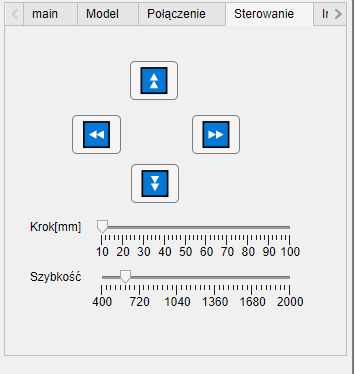
\includegraphics[height=6.5cm]{pages/siecIRobot/zdjecia/program/programUstSterowanie.png}
	\caption{Ustawienia połączeń oraz ręczne sterowanie robotem}
\end{figure}
Lewy zrzut ekranu przedstawia zakładkę pozwalającą na ustawienia połączenia pomiędzy aplikacją, a robotem i kamerą. 
Po połączeniu użytkownik ma możliwość wysłania własnej komendy G-Code wprowadzonej w odpowiednim polu. 
Dane odebrane po wysłaniu polecenia wyświetlane są w polu logów. Ekran z prawej strony po wybraniu prędkości i przesunięcia
pozwala na ręczne sterowanie karetką robota.
\begin{figure}[H]
	\centering
	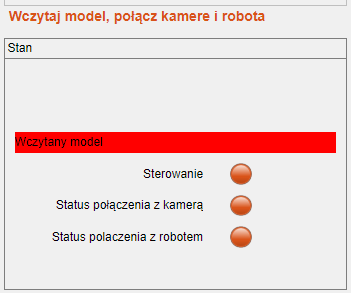
\includegraphics[height=6cm]{pages/siecIRobot/zdjecia/program/programStanErr.png}
	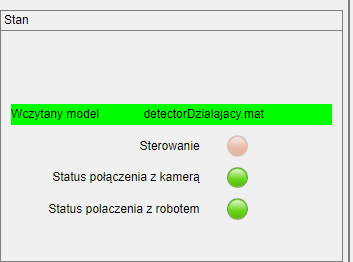
\includegraphics[height=6cm]{pages/siecIRobot/zdjecia/program/programStan.png}
	\caption{Stan aplikacji}
\end{figure}
Stan aplikacji jest cały czas prezentowany przy pomocy prostych kontrolek zmieniających swój kolor. 
Wczytanie modelu z siecią sygnalizowane jest poprzez zielony kolor i nazwę wczytanego pliku. 
Podobnie poprzez kolor sygnalizowany jest stan połączenia z robotem i zamocowaną na nim kamerą.
Kontrolka 'Sterowanie' informuje o tym, czy uruchomiony jest algorytm śledzący wybrany obiekt. 
Ostatecznie aplikacja została skompilowana do wykonywalnego pliku exe, który można uruchomić na dowolnym komputerze.
\subsection{Generowanie komend i sterowanie robotem}
Program posiada dwa różne tryby sterowania. Pierwszy tryb, po uruchomieniu algorytmu szuka wybranego obiektu, a po 
jego znalezieniu wyznacza różnicę pomiędzy środkiem obrazu, a zaznaczoną ramką i jednorazowo wysyła komendę G-Code.
Tryb "śledzenia", w przeciwieństwie do poprzedniego cały czas uruchamia sieć neuronową rozpoznającą obiekty i
wyznacza komendy odpowiadające za niewielkie przesunięcia. 
Tryb ten nazwany jest śledzącym, ponieważ dynamicznie reaguje na zmianę pozycji danego obiektu i stale za nim podąża.
\lstinputlisting[language=Matlab,caption=Uczenie sieci, label=kod:listingAlgorytmu]{pages/siecIRobot/kodSkryptu.m}
Program z listingu \ref{kod:listingAlgorytmu}, odpowiada za algorytm śledzący obiekty znalezione przez sieć neuronową. 
Niezależnie od trybu śledzenia wywoływana jest funkcja mainLoop, która odpowiada za pobranie
obrazu z kamery, uruchomienie odpowiedniej wersji algorytmu oraz dodanie do finalnego obrazu 'celownika', 
dodającego punkt odniesienia względem środka. W przypadku prostszej wersji, uruchamiana jest detekcja obiektów przy pomocy 
sieci neuronowej aż do momentu wykrycia pożądanej klasy. Po wykryciu obiektu algorytm wyznacza potrzebne do osiągnięcia celu przesunięcie, 
a następnie odpowiednio przygotowane polecenie wysyła do robota. Przesunięcie wyznaczane jest na podstawie różnicy 
środka obrazu i wykrytego obiektu, ten błąd dalej wzmacniany jest poprzez odpowiednie nastawy P1 i P2. 
Jak widać jest to regulator typu P, a współczynniki wzmocnień proporcjonalnych odzwierciedlają skalę pomiędzy obrazem, a rzeczywistą odległością.
Tryb śledzenia różni się tym, że sieć neuronowa uruchamiana jest ciągle i dzięki temu robot może nieustannie korygować błąd nadążania. 
Poza tym wyznaczone maksymalne przesunięcie ograniczone jest do stałej wartości tak, aby robot nie wykonywał zbyt dużych niepotrzebnych ruchów. 